\PassOptionsToPackage{unicode=true}{hyperref} % options for packages loaded elsewhere
\PassOptionsToPackage{hyphens}{url}
%
\documentclass[]{book}
\usepackage{lmodern}
\usepackage{amssymb,amsmath}
\usepackage{ifxetex,ifluatex}
\usepackage{fixltx2e} % provides \textsubscript
\ifnum 0\ifxetex 1\fi\ifluatex 1\fi=0 % if pdftex
  \usepackage[T1]{fontenc}
  \usepackage[utf8]{inputenc}
  \usepackage{textcomp} % provides euro and other symbols
\else % if luatex or xelatex
  \usepackage{unicode-math}
  \defaultfontfeatures{Ligatures=TeX,Scale=MatchLowercase}
\fi
% use upquote if available, for straight quotes in verbatim environments
\IfFileExists{upquote.sty}{\usepackage{upquote}}{}
% use microtype if available
\IfFileExists{microtype.sty}{%
\usepackage[]{microtype}
\UseMicrotypeSet[protrusion]{basicmath} % disable protrusion for tt fonts
}{}
\IfFileExists{parskip.sty}{%
\usepackage{parskip}
}{% else
\setlength{\parindent}{0pt}
\setlength{\parskip}{6pt plus 2pt minus 1pt}
}
\usepackage{hyperref}
\hypersetup{
            pdftitle={Causality and Multiple Regression Supplement},
            pdfauthor={Authors TBD},
            pdfborder={0 0 0},
            breaklinks=true}
\urlstyle{same}  % don't use monospace font for urls
\usepackage{longtable,booktabs}
% Fix footnotes in tables (requires footnote package)
\IfFileExists{footnote.sty}{\usepackage{footnote}\makesavenoteenv{longtable}}{}
\usepackage{graphicx,grffile}
\makeatletter
\def\maxwidth{\ifdim\Gin@nat@width>\linewidth\linewidth\else\Gin@nat@width\fi}
\def\maxheight{\ifdim\Gin@nat@height>\textheight\textheight\else\Gin@nat@height\fi}
\makeatother
% Scale images if necessary, so that they will not overflow the page
% margins by default, and it is still possible to overwrite the defaults
% using explicit options in \includegraphics[width, height, ...]{}
\setkeys{Gin}{width=\maxwidth,height=\maxheight,keepaspectratio}
\setlength{\emergencystretch}{3em}  % prevent overfull lines
\providecommand{\tightlist}{%
  \setlength{\itemsep}{0pt}\setlength{\parskip}{0pt}}
\setcounter{secnumdepth}{5}
% Redefines (sub)paragraphs to behave more like sections
\ifx\paragraph\undefined\else
\let\oldparagraph\paragraph
\renewcommand{\paragraph}[1]{\oldparagraph{#1}\mbox{}}
\fi
\ifx\subparagraph\undefined\else
\let\oldsubparagraph\subparagraph
\renewcommand{\subparagraph}[1]{\oldsubparagraph{#1}\mbox{}}
\fi

% set default figure placement to htbp
\makeatletter
\def\fps@figure{htbp}
\makeatother

\usepackage{booktabs}
\usepackage[]{natbib}
\bibliographystyle{apalike}

\title{Causality and Multiple Regression Supplement}
\author{Authors TBD}
\date{2021-03-06}

\begin{document}
\maketitle

{
\setcounter{tocdepth}{1}
\tableofcontents
}
\hypertarget{preface}{%
\chapter*{Preface}\label{preface}}
\addcontentsline{toc}{chapter}{Preface}

This textbook supplement is an introduction to causality in statistics and multivariable methods for students in their first college course in statistics. Traditionally, except for a terse warning from instructors that ``correlation does not imply causation'', students only encounter causality in statistics if they take graduate-level courses in certain disciplines (economics, epidemiology, etc.). However, given the ubiquity of data-driven arguments in modern society, a deeper understanding of drawing cause-and-effect conclusions from data is a core competency of college graduates and deserves attention in the liberal arts curriculum. For more on causality in the undergraduate curriculum, see our paper \citep{cummiskey2020causal} and others on this subject \citep{horton2015challenges, kaplan2018teaching, lubke2020we}.

Prediction and cause-and-effect are the two main scientific goals of studies employing multiple regression. Importantly, researchers use and interpret regression models differently depending upon the goal. However, this distinction is rarely made in introductory courses. Too often, multiple regression in the introductory course focuses on prediction and much of the ``thinking'' outsourced to algorithmic searches. This narrow focus on prediction deprives students of the opportunity to exercise critical judgement and creativity. On the other hand, cause-and-effect studies require tying subject matter knowledge to developing causal models. During this process, students have to carefully consider relationships between variables (which is not particularly important in prediction), thus developing multivariable thinking, an important goal of the revised GAISE report \citep{carver2016guidelines}. Our approach to multiple regression emphasizes the scientific goal of the study and how it motivates researchers' thinking about their data and models. \citet{hernan2019second} argue for this approach in data science education; we believe it is appropriate for introductory statistics courses also.

(add a mention to the revised GAISE report.)

\hypertarget{introduction}{%
\chapter{Introduction}\label{introduction}}

\hypertarget{goals-of-quantitative-research-describe-predict-cause-and-effect}{%
\section{Goals of quantitative research (describe, predict, cause-and-effect)}\label{goals-of-quantitative-research-describe-predict-cause-and-effect}}

Researchers and practitioners in nearly every discipline employ quantitative methods to answer important questions and make decisions. Regardless if it is finance, medicine, psychology, etc., all researchers typically have one of three goals \citep{cozby2020methods} when they conduct quantitative research:

\begin{itemize}
\item
  \textbf{describe}
\item
  \textbf{predict}
\item
  \textbf{cause-and-effect}
\end{itemize}

(discuss external and internal validity here?)

For example, consider medical researchers investigating a newly discovered variant of the coronavirus. Initially, they focus on describe studies. \emph{How prevalent is the variant in the population? How does the prevalence vary over space and time? What groups of individuals are most vulnerable to the variant? What else is associated with the variant?} Together, these studies help the researchers better understand the variant and identify important variables for refined predict studies.

Predict studies identify individuals most at risk for the variant or for transmitting it to others. Researchers select potential predictors as inputs to algorithms and statistical methods that transform them into estimates of each individual's risk for the variant. These methods rely upon associations between the inputs and the variant. In addition, these methods estimate the error associated with their predictions. Researchers try to ensure error estimates obtained within their study are good estimates of the error when their methods are applied to other populations. While predict studies help us identify who is at risk, they do not tell us the effect on their risk if we change something about them (quitting smoking, lost weight, etc.) To answer these ``what if?'' questions, researchers use cause-and-effect studies.

Cause-and-effect studies try to estimate the effect of intervening or changing some aspect of an individual. These studies are tremendously important in public policy (where they are aptly called \emph{intervention studies}) to justify expensive legislation and regulations to reduce risk. Unlike prediction studies, which are highly algorithmic and only require researchers to identify appropriate inputs, cause-and-effect studies use subject matter knowledge of the causal structure of the inputs to select appropriate statistical models \citep{hernan2019second}. For example, to assess the affect of quitting smoking on coronavirus risk, we would have to understand why some people quit smoking and others do not, as these reasons themselves may be responsible for some of the reduction in risk we observe between the two groups. Also, unlike prediction studies which rely upon what we \emph{see}, cause-and-effect studies require us to ask what would happen if we \emph{do} something \citep{pearl2018book}. Only human beings are capable of such counterfactual thinking (``what would have happened if'') - even our most sophisticated computer algorithms require human supervision to address cause-and-effect questions.

\textbf{Exercises}

\begin{enumerate}
\def\labelenumi{\arabic{enumi}.}
\tightlist
\item
  For the following studies, identify the goal (describe, predict, cause-and-effect) of the study. Briefly explain your choice:
\end{enumerate}

\begin{itemize}
\item
  \emph{A researcher obtains school records to collect information on the extracurricular activities of students.}
\item
  \emph{A researcher obtains school records to determine the impact of extracurricular activities on grades.}
\item
  \emph{A researcher obtains school records on extracurricular activities to identify students who are at risk to graduate.}
\end{itemize}

\begin{enumerate}
\def\labelenumi{\arabic{enumi}.}
\setcounter{enumi}{1}
\tightlist
\item
  Select an area of interest to you. Write a sentence describing a study in your area of interest for each of the three goals (describe, predict, cause-and-effect)
\end{enumerate}

\hypertarget{why-multiple-regression}{%
\section{Why multiple regression?}\label{why-multiple-regression}}

(need to edit the below from an email)

You are investigating the relationship between education and adult earnings. (Note this is almost always an observational study -- a survey of sampled individuals with variables such as income, education, age, sex, etc.)

Let's assume you've never taken our course (or one like it). You can get pretty far investigating this data with concepts most students learn in high school. For example, you could compare adult earnings in college graduates to those of non-college graduates or find an estimate of earnings per year of education. If you are especially savy, you might recognize that college graduates and noncollege graduates are different in ways (age, sex, etc.) that are also important to adult earnings and repeat your original analyses within the different levels of these variables. To you (and most people outside our discipline), statistics is arithmetic, and it is hard to envision anything beyond arithmetic if that's all you know. However, there are important questions you cannot answer with this limited view of statistics:

\begin{enumerate}
\def\labelenumi{(\arabic{enumi})}
\item
  What range of population values for measures of association between education and adult earnings are compatible with your data?
\item
  If there is no association between education and earnings, how extreme are your observed results?
\item
  What is the association between education and earnings holding other important variables constant?
\item
  How does the relationship between education and earnings depend upon other variables?
\end{enumerate}

Most people's cynicism towards statistics is rooted in a lack of understanding that our discipline has answers to (1)-(4).

Thus far in our course, we have focused on (1) and (2) for various types of independent and dependent variables. And, if someone were to ask me, ``what have your students learned in your course this semester?'', my response would start with (1) and (2). These are important concepts\ldots{}humans are not predisposed to think this way.

However, you still cannot answer (3) and (4) if you're in our course right now. (3) relates to confounding; (4) is interactions. The concepts of confounding and interactions are best understood before approaching multiple regression (a point we discuss at length here: \url{https://www.overleaf.com/read/nkzpvpxwsjzq}). However, multiple regression is the most flexible statistical model for estimating quantities in (3) and (4). Being able to answer (3) and (4) is a huge step up in a student's capability. Comparing earnings of college graduates to noncollege graduates is meaningless if these groups are vastly different with regards to age, sex, etc. Unless you have formal education in these methods, you probably don't know (3) and (4) are possible -- it's outside what you can do with arithmetic.

Okay, so that's some discussion on why do we teach multiple regression? Now, what do we teach about multiple regression?

Broadly speaking, there are two major aspects to multiple regression: theory, application. Given our students and where this course fits into their education, I am an unabashed proponent of application being the primary focus of our course.

Examples of theory - derive the least squares estimates of the regression coefficients, understand the geometric interpretation of regression, etc.

Examples of application - fit and interpret a model to estimate the association between education and earnings that adjusts for age.

You can have a rich understanding of one of these two aspects and be a complete novice about the other. From my experience, mathematicians are rock stars in theory but haven't seen as much application (don't worry, you have more than enough for this course). For example, in application, a statistician would employ multiple regression in very different ways depending on whether the primary goal of the study is (a) prediction or (b) estimating the effect of an intervention. In (a), the primary concern is making smart use of the data to obtain ``good'' estimates of the out-of-sample prediction error with little care to what's in the model. In (b), the primary concern is confounding, which is a type of statistical bias, so variables are selected carefully by the researcher to reflect the intervention of interest. The distinction between (a) and (b) is beyond the scope of our course, but I'm just trying to illustrate the richness there is to both the theory and application of multiple regression.

So, back to our course, I think the Michigan house prices example in Intermediate Statistical Analyses by Tintle et. al.~and Dan Baller's worksheet sums up well what I think students should get from our course. Specifically, they should get an appreciation that there are statistical models that (1) estimate measures of association while holding other variables constant and (2) see how these associations change based on other variables. For (2), an interaction between a quantitative and categorical variable is about as far as we can reasonably expect most students to get.

\hypertarget{causality}{%
\chapter{(Kevin) Causality}\label{causality}}

\hypertarget{what-does-it-mean-for-one-thing-to-cause-another}{%
\section{What does it mean for one thing to cause another}\label{what-does-it-mean-for-one-thing-to-cause-another}}

\hypertarget{randomized-controlled-experiments}{%
\section{Randomized controlled experiments}\label{randomized-controlled-experiments}}

\hypertarget{observational-studies}{%
\section{Observational Studies}\label{observational-studies}}

\hypertarget{confounding}{%
\section{Confounding}\label{confounding}}

\hypertarget{causal-diagrams}{%
\section{Causal Diagrams}\label{causal-diagrams}}

\hypertarget{matching}{%
\chapter{Matching}\label{matching}}

Chapter on matching

\hypertarget{categorical}{%
\chapter{(COL Watts) Quantitative explanatory variable with categorical confounding variable}\label{categorical}}

Introduce multiple regression by adding a categorical confounding variable

Explanatory (\(X\)) - quantitative

Response (\(Y\)) - quantitative

Confounding (\(C\)) - categorical

\hypertarget{unadjusted-effect-of-x-on-y}{%
\section{\texorpdfstring{Unadjusted effect of \(X\) on \(Y\)}{Unadjusted effect of X on Y}}\label{unadjusted-effect-of-x-on-y}}

short review of simple regression

\hypertarget{effect-of-x-and-y-adjusting-for-c.}{%
\section{\texorpdfstring{Effect of \(X\) and \(Y\) adjusting for \(C\).}{Effect of X and Y adjusting for C.}}\label{effect-of-x-and-y-adjusting-for-c.}}

\hypertarget{assessing-model-adequacy}{%
\section{Assessing model adequacy}\label{assessing-model-adequacy}}

\hypertarget{interactions}{%
\chapter{(Kevin) Interactions}\label{interactions}}

Extend the example in the last chapter\ldots{}introduce in terms of effect modification. We have a new research question, ``does the affect of \(X\) on \(Y\) change based on another variable of interest?''

\hypertarget{activity}{%
\chapter{Activity}\label{activity}}

\emph{Title}: The Indoor Obstacle Course Test (IOCT)

\emph{Topics}\}*: Confounding, Causal Diagrams, Simple Linear Regression, Confidence Intervals

\emph{Background}: Cadets at West Point must pass the \href{https://www.youtube.com/watch?v=94tPO0fGtJo\&t=77s}{Indoor Obstacle Course Test} (IOCT) to graduate. The IOCT begins with a series of floor and climbing obstacles and ends with several laps around an indoor track. It is an exhausting test of endurance and strength. In addition to being a graduation requirement, cadets receive a letter grade that is factored into their class rank.

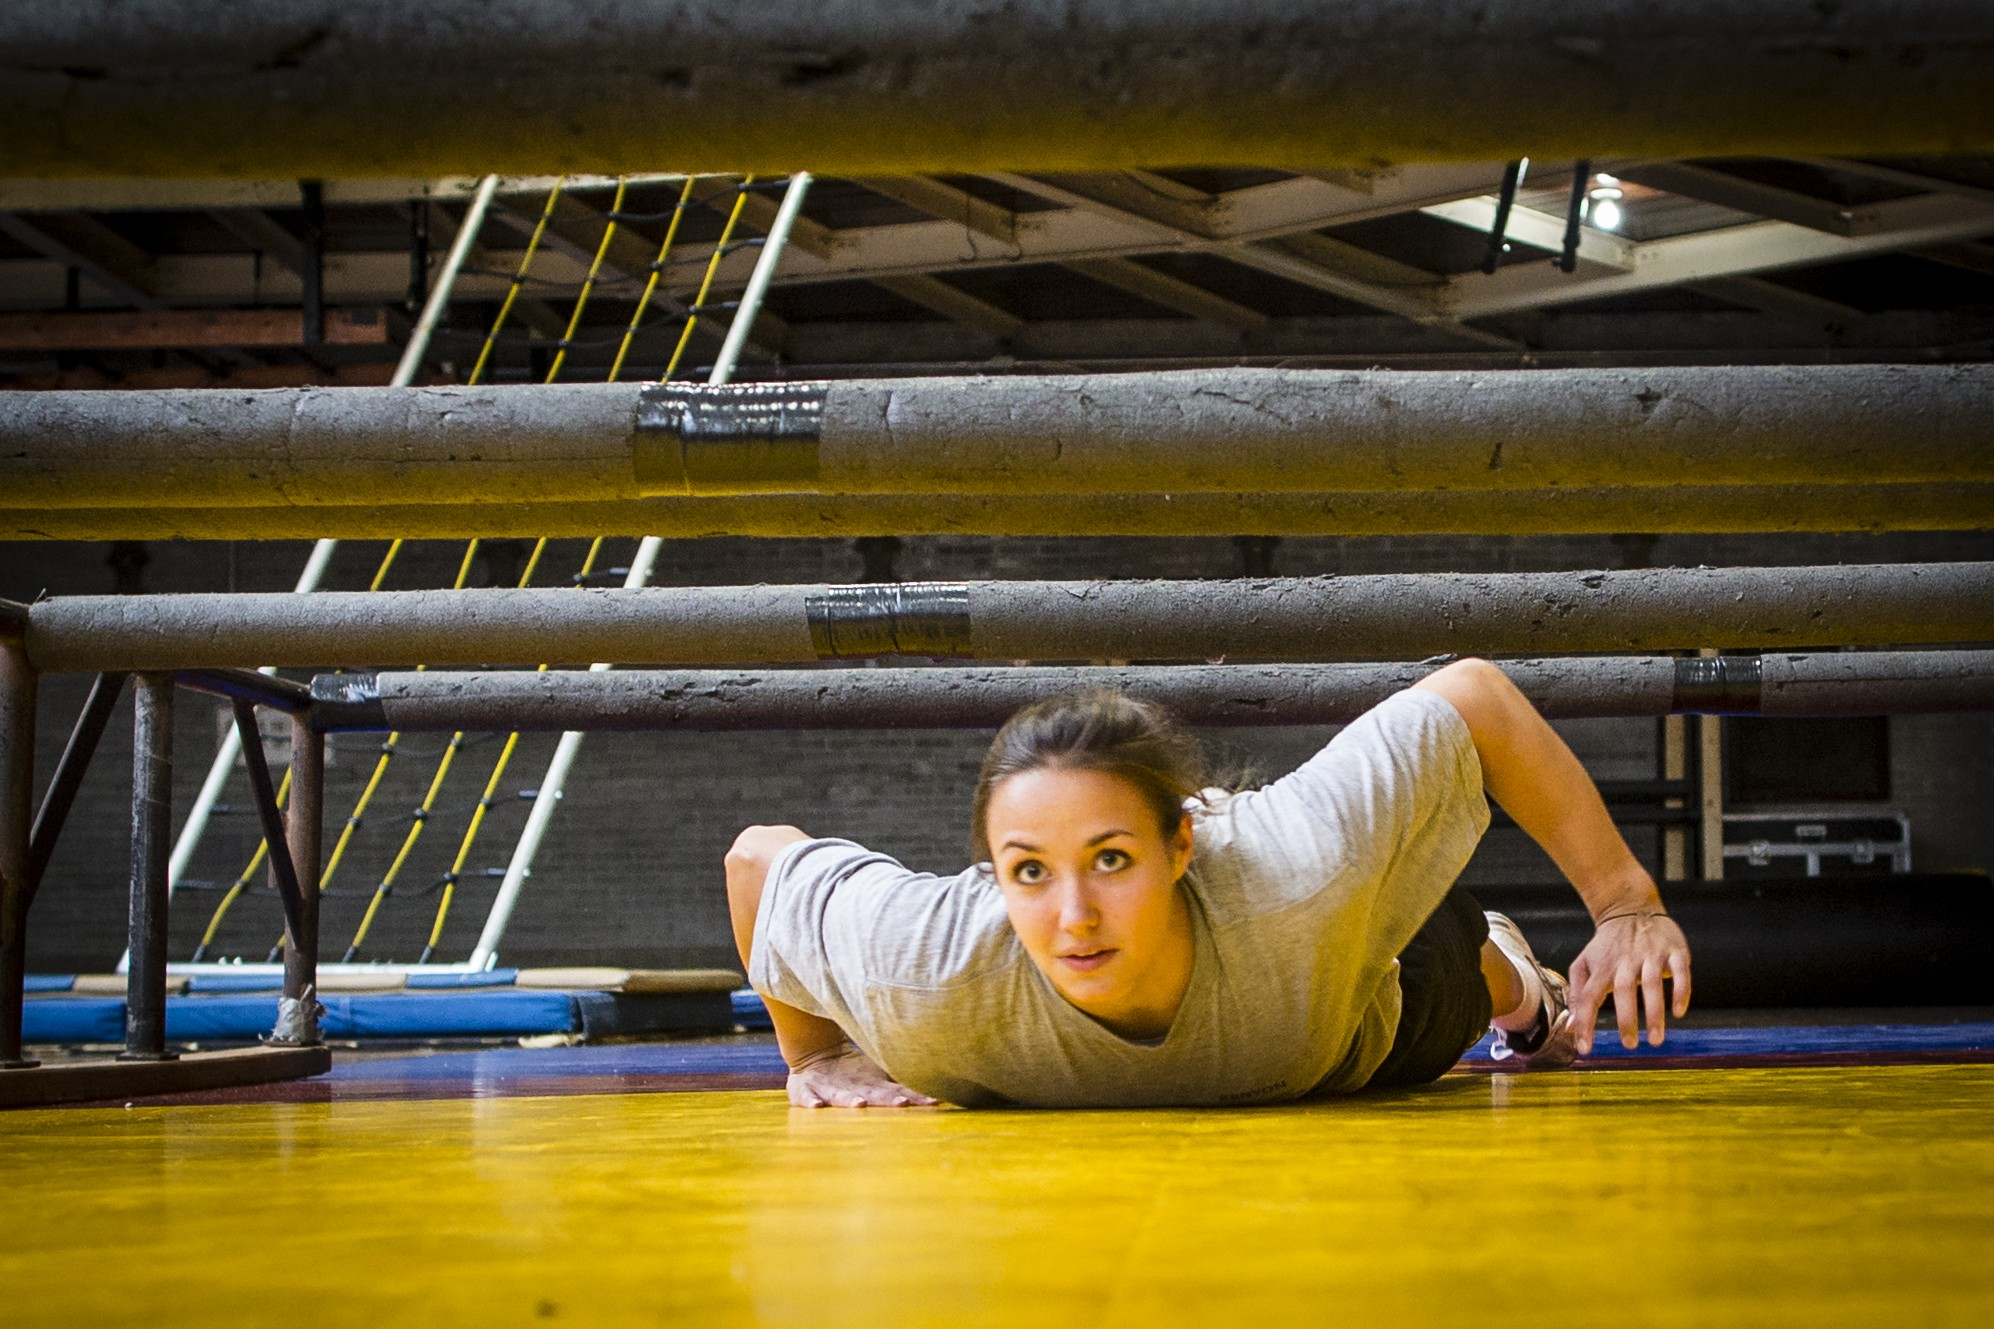
\includegraphics[width=0.5\textwidth,height=\textheight]{./images/crawlObstacle.jpg} 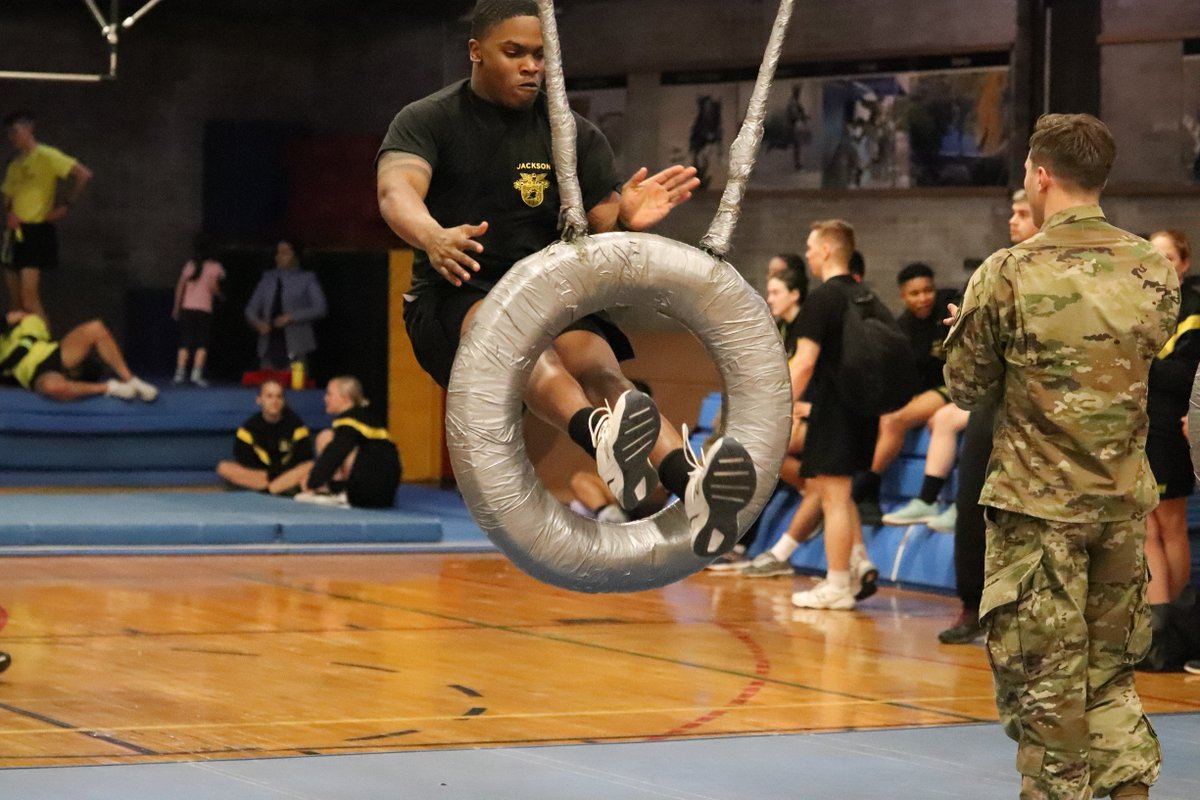
\includegraphics[width=0.5\textwidth,height=\textheight]{./images/tireObstacle.jpg}

Shorter cadets often argue they are at a disadvantage on the obstacle course. Many obstacles appear to favor taller cadets because they are easier to reach. In this study, we will investigate the effect of height on IOCT times.

\begin{enumerate}
\def\labelenumi{\arabic{enumi}.}
\tightlist
\item
  \href{https://www.youtube.com/watch?v=94tPO0fGtJo\&t=77s}{Watch the video of Cadet Madaline Kenyon running the IOCT}. In your opinion, do some obstacles favor taller cadets? Explain.
\end{enumerate}

\vspace{1in}

The file \texttt{obstacle\_course.csv} contains height (inches), IOCT times (seconds), biological sex (M/F), and whether the cadet played an intercollegiate sport for a sample of 384 cadets who ran the IOCT course in the last five years.

\begin{enumerate}
\def\labelenumi{\arabic{enumi}.}
\setcounter{enumi}{1}
\tightlist
\item
  What is the explanatory variable in this study? Classify the variable as quantitative or categorical.
\end{enumerate}

\vspace{0.25in}

\begin{enumerate}
\def\labelenumi{\arabic{enumi}.}
\setcounter{enumi}{2}
\tightlist
\item
  What is the response variable in this study? Classify the variable as quantitative or categorical.
\end{enumerate}

\vspace{0.25in}

\begin{enumerate}
\def\labelenumi{\arabic{enumi}.}
\setcounter{enumi}{3}
\tightlist
\item
  Is this study an observational study or a randomized experiment? Explain.
\end{enumerate}

\vspace{1in}

\newpage

Figure 1 depicts IOCT times in seconds versus height in inches. Table 1 contains information from the linear regression model.

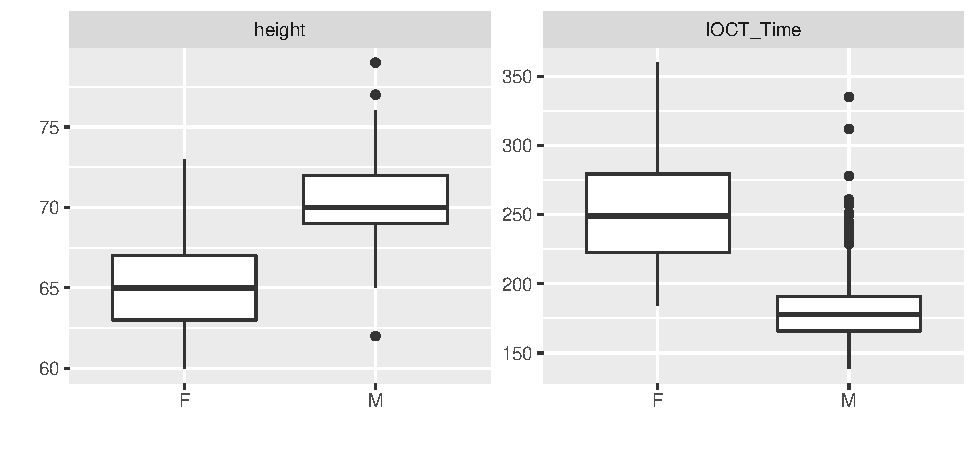
\includegraphics{MA206supplement_files/figure-latex/unnamed-chunk-3-1.pdf}

\begin{table}

\caption{\label{tab:unnamed-chunk-3}Linear regression output for IOCT times and height.}
\centering
\begin{tabular}[t]{l|r|r|r|r}
\hline
term & estimate & std.error & statistic & p.value\\
\hline
(Intercept) & 621.00 & 39.98 & 15.53 & 0\\
\hline
height & -6.08 & 0.58 & -10.52 & 0\\
\hline
\end{tabular}
\end{table}

\begin{enumerate}
\def\labelenumi{\arabic{enumi}.}
\setcounter{enumi}{4}
\item
  Interpret the estimate of the height coefficient in Table 1.

  \vspace{1in}
\item
  Calculate and interpret a 95\% confidence interval for the slope coefficient.
\end{enumerate}

\vspace{1in}

\newpage

\begin{enumerate}
\def\labelenumi{\arabic{enumi}.}
\setcounter{enumi}{6}
\tightlist
\item
  The \(p\)-value for height in Table 1 indicates there is strong evidence of an association between height and IOCT time. Taller cadets tend to do better on the IOCT. Some people would say the result is \emph{statistically significant}. However, statistical significance and practical signifigance are different. \href{https://en.wikipedia.org/wiki/Indoor_Obstacle_Course_Test}{Review the grade scale for the IOCT.} In your opinion, does the observed association have practical significance? Explain.
\end{enumerate}

\vspace{1in}

\begin{enumerate}
\def\labelenumi{\arabic{enumi}.}
\setcounter{enumi}{7}
\tightlist
\item
  A shorter cadet argues Figure 1 shows evidence the IOCT is unfair based on height. Do you agree or disagree? Explain.
\end{enumerate}

\vspace{1in}

\begin{enumerate}
\def\labelenumi{\arabic{enumi}.}
\setcounter{enumi}{8}
\tightlist
\item
  Briefly explain the difference between these two conclusions.
\end{enumerate}

\begin{itemize}
\item
  \emph{Height is associated with faster IOCT times.}
\item
  \emph{Height causes faster IOCT times.}
\end{itemize}

\vspace{1in}

\begin{enumerate}
\def\labelenumi{\arabic{enumi}.}
\setcounter{enumi}{9}
\tightlist
\item
  Based on the analysis presented thus far, is it possible to distinguish between these two explanations? Explain.
\end{enumerate}

\vspace{1in}

\begin{enumerate}
\def\labelenumi{\arabic{enumi}.}
\setcounter{enumi}{10}
\tightlist
\item
  Draw a causal diagram depicting the relationship between height, IOCT time, and sex. Explain your decisions to include/exclude arrows in the diagram.
\end{enumerate}

\vspace{1in}

\begin{enumerate}
\def\labelenumi{\arabic{enumi}.}
\setcounter{enumi}{11}
\tightlist
\item
  Based on your diagram, identify the confounding variable.
\end{enumerate}

\vspace{0.5in}

Below are boxplots of height in inches and IOCT times in seconds by sex.

\begin{figure}
\centering
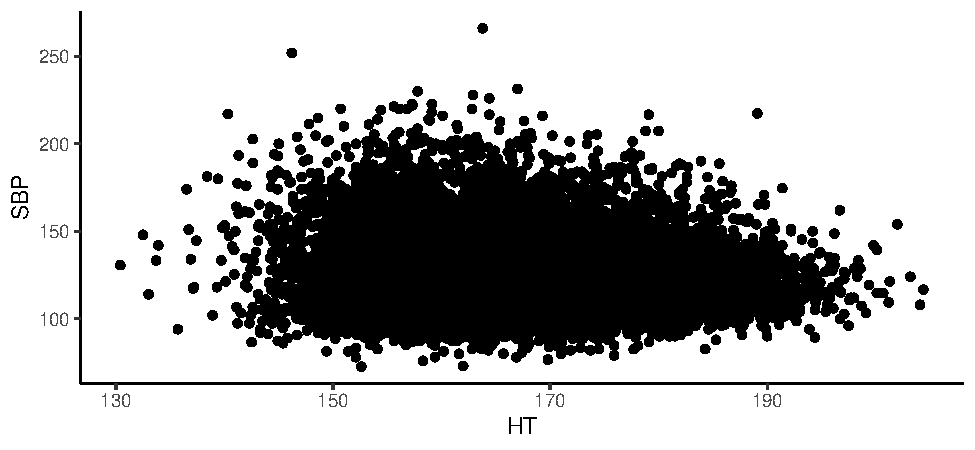
\includegraphics{MA206supplement_files/figure-latex/unnamed-chunk-4-1.pdf}
\caption{\label{fig:unnamed-chunk-4}Height (inches) and IOCT time (seconds) by sex.}
\end{figure}

\begin{enumerate}
\def\labelenumi{\arabic{enumi}.}
\setcounter{enumi}{12}
\tightlist
\item
  Based on Figure 2, is the estimate of the effect of height on IOCT time in Table 1 confounded by sex? If so, is the effect of height smaller or larger than that reported in Table 1? Explain.
\end{enumerate}

\vspace{1in}

\newpage

Figure 3 depicts the association between IOCT time and height by sex. Tables 2 and 3 depict regression results for female and male cadets, respectively.

\begin{figure}
\centering
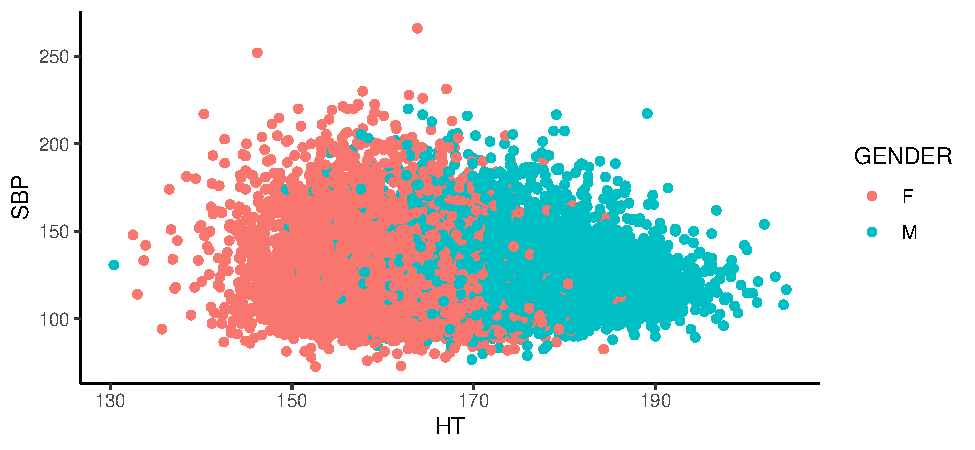
\includegraphics{MA206supplement_files/figure-latex/unnamed-chunk-5-1.pdf}
\caption{\label{fig:unnamed-chunk-5}Indoor Obstacle Course Test (IOCT) times versus height by sex (n = 384).}
\end{figure}

\begin{table}

\caption{\label{tab:unnamed-chunk-6}Regression results for female cadets.}
\centering
\begin{tabular}[t]{l|r|r|r|r}
\hline
term & estimate & std.error & statistic & p.value\\
\hline
(Intercept) & 335.76 & 107.44 & 3.12 & 0.00\\
\hline
height & -1.24 & 1.64 & -0.76 & 0.45\\
\hline
\end{tabular}
\end{table}

\begin{table}

\caption{\label{tab:unnamed-chunk-6}Regression results for male cadets.}
\centering
\begin{tabular}[t]{l|r|r|r|r}
\hline
term & estimate & std.error & statistic & p.value\\
\hline
(Intercept) & 175.61 & 40.92 & 4.29 & 0.00\\
\hline
height & 0.09 & 0.58 & 0.15 & 0.88\\
\hline
\end{tabular}
\end{table}

\begin{enumerate}
\def\labelenumi{\arabic{enumi}.}
\setcounter{enumi}{13}
\tightlist
\item
  Based on Figure 3 and Tables 2 and 3, does it appear there is an association between IOCT time and height within levels of sex? Explain.
\end{enumerate}

\vspace{1in}

\newpage

\begin{enumerate}
\def\labelenumi{\arabic{enumi}.}
\setcounter{enumi}{14}
\tightlist
\item
  In your opinion, is there much evidence that height is an advantage on the IOCT (in other words, is height the \emph{cause} of better IOCT times)? Explain.
\end{enumerate}

\vspace{2in}

\begin{enumerate}
\def\labelenumi{\arabic{enumi}.}
\setcounter{enumi}{15}
\tightlist
\item
  Briefly discuss two ways you could improve this study to better assess whether there is a height advantage.
\end{enumerate}

\vspace{1in}

\hypertarget{quantitative}{%
\chapter{(COL Watts) Quantitative explanatory variable with quantitative confounding variable}\label{quantitative}}

Explanatory (\(X\)) - quantitative

Response (\(Y\)) - quantitative

Confounding (\(C\)) - quantitative

\hypertarget{effect-of-x-and-y-adjusting-for-c.-1}{%
\section{\texorpdfstring{Effect of \(X\) and \(Y\) adjusting for \(C\).}{Effect of X and Y adjusting for C.}}\label{effect-of-x-and-y-adjusting-for-c.-1}}

\hypertarget{assessing-model-adequacy-1}{%
\section{Assessing model adequacy}\label{assessing-model-adequacy-1}}

\bibliography{book.bib,packages.bib}

\end{document}
